\documentclass[main]{subfiles}
\begin{document}

%@@@@@@@@@@@@@@@@@@@@@@@@@@@@@@
% Main Topics: Neural Code 25.10.2018
% Lecturer: Benjamin Grewe
% author: Vanessa Leite - base document from benelot/eth-intro-to-neuroinformatics-summary

\section{Neural Coding}

The problem we are trying to elucidate with neural coding is ``the representation and transformation of information in the nervous system".
To better understand this, we need to work with four concepts:

\paragraph{Correspondence} a code is the correspondence between two domains. This mean that one domain (for instance, visual signal) can be specified (encoded) by another (for instance, spike trains), this way one can, theoretically, reconstruct  the original message from the encoded message with some accuracy (decoding).

\paragraph{Representation} not all cases of correlation are considered as a instance of coding.

\paragraph{Causality} Although spike trains encode visual signal, we wouldn't say that visual signals enconde spike trains. This is because we assume a casual relation: visual signals generate (cause) spike trains.

\paragraph{Encoding} How does a stimulus cause a pattern of responses? Building an approximate mechanistic model of the world.

\paragraph{Decoding} What do the responses tell us about the stimulus? How can we reconstruct the stimulus?
By recording neuronal responses in the cat visual cortex, we identify that the visual cortex encondes the orientation of a moving stimulus and has a orientation specific organization.
In rats, spatial information is coded via hippocampal place cells.

\paragraph{General}

\begin{itemize}[noitemsep,nolistsep]
	\item Information is encoded by firing of single neurons and firing of populations of neurons.
	\item A neuron encodes information, fires to stimuli.
	\item Firing rate and spike timing encodes information.
	\item Spatial/temporal resolution of different measurement techniques tell us about the neural code.
	\item It is an issue to record from many neurons simultaneously.
	\item There is not much information in the slope of a spike.
	\item By recording neuronal responses from a stimuli, we can ``see" how the brain encodes the stimuli.
\end{itemize}

\begin{figure}[H]
	\centering
	\begin{subfigure}[b]{0.5\textwidth}
		\centering
		\includegraphics[width=\textwidth]{neural-coding-problem.png}
	\end{subfigure}%
	~
	\begin{subfigure}[b]{0.5\textwidth}
		\centering
		\includegraphics[width=\textwidth]{firing-rate.png}
	\end{subfigure}
\end{figure}

\begin{itemize}[noitemsep,nolistsep]
	\item Raster plot with spikes and histogram. Stimulus takes place at $t = 0$.
	\item Use bins (about 100 ms in time) with a sliding window and a gauss filter and causal filter.
	\item Problematic are intermediate stages, probability of firing, background activity and varying membrane potentials.
	\item Causal filter is $w(\tau) = [\alpha^2\tau\exp(-\alpha\tau)]$
	\item Typically neurons fire between $1\,Hz$ and $200\,Hz$ - often around $40\,Hz$.
\end{itemize}



\subsection{Neuronal Rate Codes}
Rate coding refers to information being carried by the firing rate. It is often
argued, or assumed, that firing rate captures essentially all relevant information.

\begin{itemize}[noitemsep,nolistsep]
	\item Rate = average over time, single neuron, single run.
	\item $v = \frac{n_{sp}}{T}$
	\item Definition of the mean firing rate via a temporal average.
	\item Neuronal gain function (curve). The output spike rate is given as a function of the total somatic input current $I_0$.
	\item Easy to understand, but no timing effects and misleading as more than one stimulus might be encoded.
	\item It takes time to compute a temporal average and behavioral response time is shorter than integration time.
\end{itemize}

\subsection{Neuronal Temporal Codes}
Temporal coding may refer to several quite different ideas:
\begin{itemize}
\item Much of the information may be transmitted by a neuron during certain small intervals of time.
\item synchronous, or what I would call quasi-synchronous, firing of neurons within and across ensembles may carry important information.
\item the precise timing, or pattern, of spikes may carry information.
\end{itemize}

\subsection{Sound localization by measuring  the Interaural Time Difference (ITD)}

\begin{figure}[H]
	\centering
	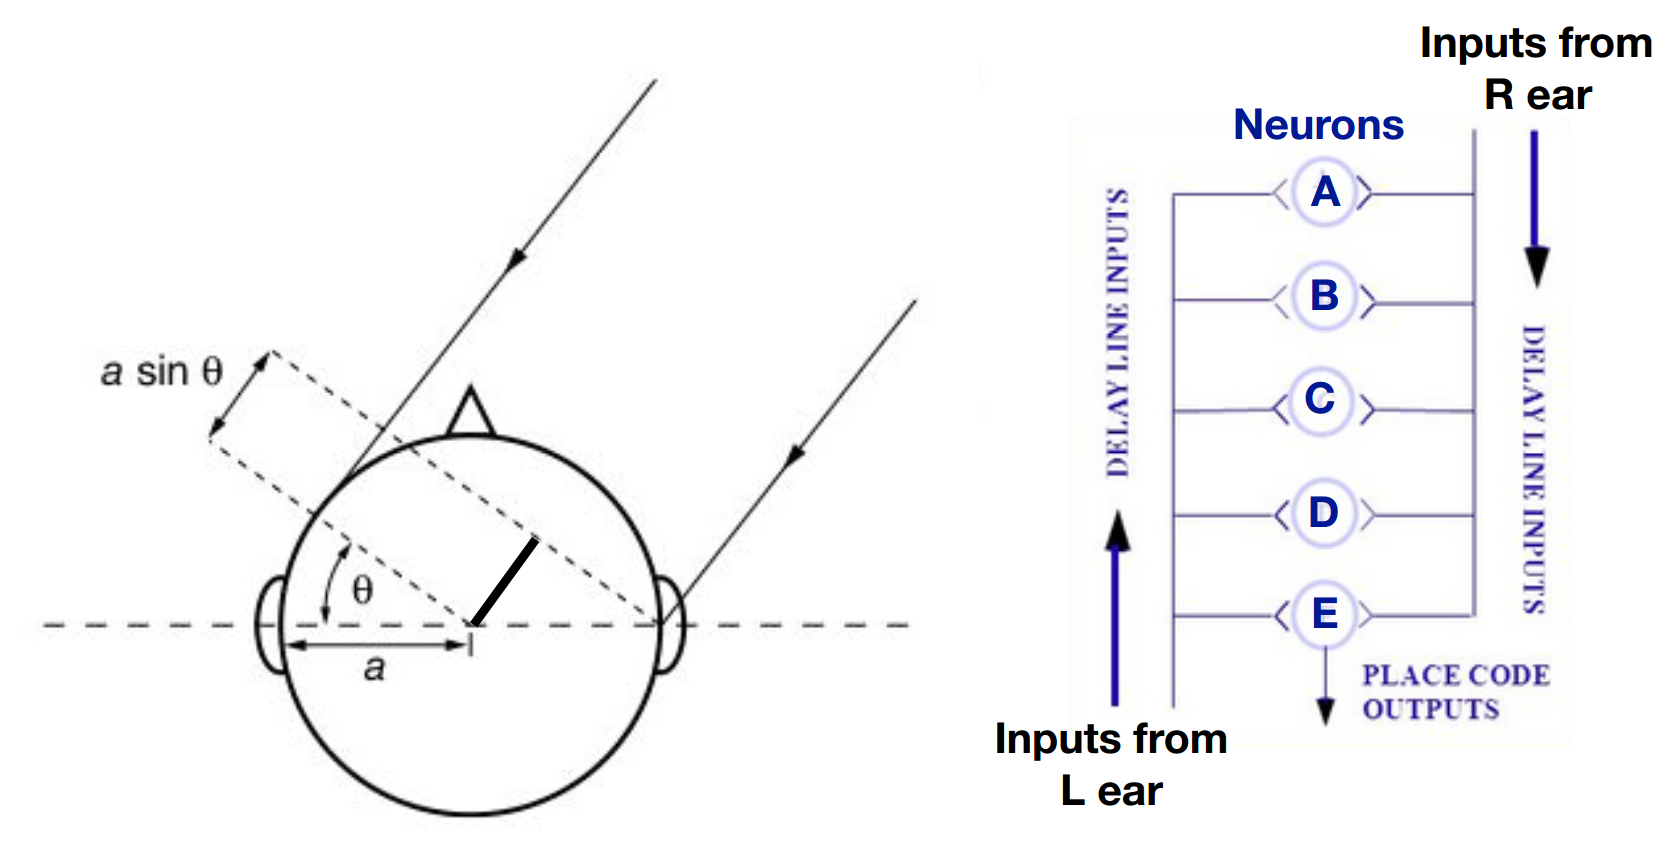
\includegraphics[width=0.7\textwidth]{interaural-time-difference.png}
\end{figure}

\subsection{Peri-Stimulus Time Histogram (PSTH)}
\begin{itemize}[noitemsep,nolistsep]
	\item $\rho = \frac{1}{\Delta t}\frac{1}{K}n_K(t;t+\Delta t)$ where $K$ is the number of trials.
	\item Spike density is an average over several runs of the experiment.
\end{itemize}

\subsection{Tuning Curves}
\begin{itemize}[noitemsep,nolistsep]
	\item Tuning curves show average firing rate response to varying stimulus parameters.
\end{itemize}
\begin{figure}[H]
	\centering
	\includegraphics[scale=0.5]{tuning-curve.png}
\end{figure}

\subsection{Orientation Maps}
\begin{itemize}[noitemsep,nolistsep]
	\item Nearby neurons have similar preferred orientations.
	\item Orientation-selective neurons (in the primary visual cortex of cats).
	\item Orientation column and pinwheels.
\end{itemize}

\subsection{Poisson Spike Trains}
\begin{itemize}[noitemsep,nolistsep]
	\item Mathematical model to describe and generate spike trains.
	\item Poission distribution for the number of spikes in interval $T$ with firing rate $r$.
	\item $P_T(n)=\frac{(rT)^n}{n!}\exp(-rT)$
	\item Homogeneous: Constant rate.
	\item Inhomogeneous: Variable rate.
	\item Approximation: Probability of a spike occurring in short interval of length $\Delta t$: $r(t)\cdot\Delta t$
\end{itemize}

\subsection{What a single neuron can encode}
\begin{itemize}[noitemsep,nolistsep]
	\item Places (on entering a particular region).
	\item Grids (regularly arranged triangular grid of locations).
	\item Head-direction, compass-like.
	\item Single cells that respond to only one person.
\end{itemize}

\subsection{Population Rates}
\begin{itemize}[noitemsep,nolistsep]
	\item Rate = average over pool of equivalent neurons (several neurons, single run).
	\item Activity $A=\frac{1}{\Delta t}\frac{n_{act}(t;t+\Delta t)}{N}$
	\item A postsynaptic neuron receives spike input from a population $m$ with activity $A_m$. The population activity is defined as the fraction of neurons that are active in a short interval $[t,t+\Delta t]$ divided by $\Delta t$.
\end{itemize}

\subsection{Population Codes}
\begin{itemize}[noitemsep,nolistsep]
	\item Different cells encode different ranges of the stimulus.
	\item Averaging over a population often meaningless.
	\item Allows accurate reconstruction of the signal, also interpolated between peaks.
	\item Sparse coding: Only few cells are activated.
	\item Retina as an example: Different cells for different light wavelengths.
	\item a neuron encodes a stimulus, a neuronal population encodes behavior.
\end{itemize}

\subsubsection{Population Vector Code}
\begin{itemize}[noitemsep,nolistsep]
	\item Population of neurons with different preferred arm movement directions.
	\item Encoded direction (arrow) corresponds to vectorial addition, weighted by firing rate.
	\item Interesting for brain-computer interfaces.
\end{itemize}

\subsubsection{Measuring Population Activity in vivo}
\begin{itemize}
\item calcium imaging
\item fmri
\end{itemize}

\subsubsection{Taking multiple stimuli into account}
Repeatedly sample responses to a variety of stimuli so that we can characterize what feature combination triggers a spike or a behavior.
\[ P(\text{response} | \text{stimulus}) = P(\text{response} | s_1, s_2, s_3, \dots , s_n ) \].
After collecting data, if we don't have any labels for the stimuli, we use an unsupervised/clustering approach, otherwise a supervised approach to identify the characteristics that trigger a behavior.

\subsection{Neuronal Event Codes}
\subsubsection{Time-to-first Spike Codes}
\begin{itemize}[noitemsep,nolistsep]
	\item High rate implies fast firing.
	\item Can implement competition among different input cells.
	\item Can be extended to rank-order codes (firing sequence of different neurons).
	\item Is very fast and efficient, has evidence in auditory, visual and somatosensory systems.
	\item Susceptible to noise, requires a reference signal.
\end{itemize}

\subsubsection{Burst- and Temporal Codes}
\begin{itemize}[noitemsep,nolistsep]
	\item Bush-cricket auditory neurons in natural environment.
	\item Preserve very high coding precision in extreme noise.
\end{itemize}
\begin{figure}[H]
	\centering
	\includegraphics[width=0.6\textwidth]{burst-code.png}
\end{figure}

\subsubsection{Oscillations and Phase Coding}
\begin{itemize}[noitemsep,nolistsep]
	\item Phase: The neurons fire at different phases with respect to the background oscillation.
	\item Phase could code relevant information.
\end{itemize}
\begin{figure}[H]
	\centering
	\includegraphics[width=0.4\textwidth]{phase-code.png}
\end{figure}

\subsubsection{Coding by Synchrony}
\begin{itemize}[noitemsep,nolistsep]
	\item Synchrony can encode information.
	\item Neurons can fire (nearly) synchronous.
\end{itemize}

\subsection{Local Field Potential (LFP)}
\begin{itemize}[noitemsep,nolistsep]
	\item Low-pass filtered extracellular recording.
	\item Reflects the integration of membrane currents in a local region.
	\item Dominated by dendritic synaptic activity.
	\item Might encode different properties of the stimulus than single cell firing.
	\item Spike sorting: Assigning spikes to different neurons from extracellular signal (spike shapes are unique for each neuron).
\end{itemize}

\subsection{fMRI}
\begin{itemize}[noitemsep,nolistsep]
	\item Functional magnetoc resonance imaging.
	\item Non-invasive technique for monitoring brain function.
	\item Based on BOLD (blood oxygenation level dependent signal change). Haemodynamic response function (HRF).
	\item Slow temporal resolution.
\end{itemize}

\subsection{Binding Problem}
\begin{itemize}[noitemsep,nolistsep]
	\item Occurs frequently: Visual processing (what, where).
	\item Potential mechanism: Temporal synchrony, hierarchical coding, population coding.
\end{itemize}

\subsection{Averages}
\begin{itemize}[noitemsep,nolistsep]
	\item Spike triggered average: Average over stimulus in short time window before spike.
	\item Sensory neurons typically respond stronger to rapid changes in stimulus properties.
\end{itemize}
\begin{figure}[H]
	\centering
	\begin{subfigure}[b]{0.5\textwidth}
		\centering
		\includegraphics[width=\textwidth]{spike-triggered-average.png}
	\end{subfigure}%
	~
	\begin{subfigure}[b]{0.5\textwidth}
		\centering
		\includegraphics[width=\textwidth]{stimulus-estimation.png}
	\end{subfigure}
\end{figure}

\subsection{Stimulus Reconstruction}
\begin{itemize}[noitemsep,nolistsep]
	\item Allows an observer to reconstruct the stimulus from spike trains.
	\item Probability and information theory is the mathematical background.
	\item Whole stimulus reconstruction may not be relevant.
	\item Evolution may have shaped us to encode particular features better than others, for example faces.
	\item Cells may respond to only particular aspects of stimulus.
	\item Cells may respond to multiple aspects of stimulus.
	\item Artificial stimuli used for studies may be predictable.
\end{itemize}



\end{document}
